\documentclass[aspectratio=169,11pt]{beamer}

% ============================================================
% SISMID 2026 -- Day 2, 1:30 session, Part 1
% From dengue exercise to ARGO (S. Yang + C. Djorno)
% Continues the dengue exercise: static vs dynamic training,
% adding terms, adding autoregression, combining AR + Google
% search = ARGO, then network approaches (ARGONet).
% Built on Mauricio's exercise 2 (MIGHTE-lab/SISMID25).
% Compile: pdflatex dengue-to-argo.tex  (run twice)
% ============================================================

\IfFileExists{beamerthememetropolis.sty}{
  \usetheme{metropolis}
  \metroset{progressbar=frametitle, sectionpage=progressbar, numbering=fraction}
}{
  \usetheme{Boadilla}
  \usecolortheme{seahorse}
  \setbeamertemplate{navigation symbols}{}
}

\usepackage[utf8]{inputenc}
\usepackage[T1]{fontenc}
\usepackage{tikz}
\usetikzlibrary{arrows.meta, positioning, fit, backgrounds, calc}
\usepackage{xcolor}
\usepackage{listings}
\usepackage{amsmath}

\definecolor{AccentA}{HTML}{2A6F97}
\definecolor{AccentB}{HTML}{C1666B}
\definecolor{AccentC}{HTML}{3B8A5B}
\setbeamercolor{frametitle}{bg=AccentA}
\setbeamercolor{progress bar}{fg=AccentB}

\definecolor{skbg}{rgb}{0.96,0.96,0.94}
\lstdefinestyle{prompt}{
  basicstyle=\ttfamily\scriptsize,
  backgroundcolor=\color{skbg},
  showstringspaces=false, breaklines=true,
  frame=single, framesep=4pt, columns=fullflexible, numbers=none,
}
\lstset{style=prompt}

\tikzset{
  cbox/.style={draw=AccentA, very thick, rounded corners, align=center,
    minimum height=1.0cm, inner sep=6pt, font=\small, fill=AccentA!6},
  sbox/.style={draw=AccentA, thick, rounded corners, align=center,
    minimum height=0.85cm, inner sep=4pt, font=\scriptsize, fill=AccentA!6},
  rbox/.style={draw=AccentB, thick, rounded corners, align=center,
    minimum height=0.85cm, inner sep=4pt, font=\scriptsize, fill=AccentB!8},
  gbox/.style={draw=AccentC, thick, rounded corners, align=center,
    minimum height=0.85cm, inner sep=4pt, font=\scriptsize, fill=AccentC!8},
  flow/.style={-{Stealth[length=3mm]}, very thick, draw=AccentB},
  flowq/.style={-{Stealth[length=2.4mm]}, thick, draw=AccentA!70},
}

\title{From the Dengue Exercise to ARGO}
\subtitle{One regression, grown step by step into a real forecaster}
\author{Shihao Yang \quad\textbullet\quad Candice Djorno}
\institute{SISMID 2026 \textbullet\ Day 2, 1:30}
\date{July 21, 2026}

\begin{document}

\begin{frame}
  \titlepage
\end{frame}

\begin{frame}{Where we pick up}
  Yesterday you fit a \textbf{static} least-squares line: dengue cases from the
  \texttt{dengue} search term, trained once on 2004--2006.
  \begin{block}{Today, four small upgrades, same dengue data}
    Static $\to$ \textbf{dynamic} training $\to$ \textbf{more terms} $\to$
    \textbf{autoregression} $=$ \textbf{ARGO}. Then borrow from neighbors (ARGONet).
  \end{block}
  \vspace{0.3em}
  \begin{itemize}
    \item It stays an \textbf{interpretable regression} the whole way. No black box.
    \item Same agent workflow: one prompt per upgrade, and you check the error each time.
    \item Continues Mauricio's exercise 2; the pieces are the same, the destination is ARGO.
  \end{itemize}
\end{frame}

\begin{frame}{Roadmap}
  \tableofcontents
\end{frame}

% ===============================================================
\section{Static vs dynamic training}

\begin{frame}{The problem with training once}
  A static model freezes the search-to-disease relationship in 2004--2006. But that
  relationship \textbf{drifts}: behavior changes, Google changes, the disease changes.
  \begin{center}
  \resizebox{0.9\textwidth}{!}{%
  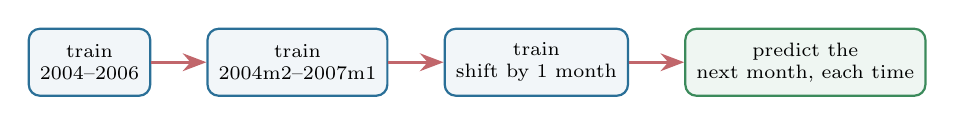
\begin{tikzpicture}[node distance=0.7cm]
    \node[sbox] (w1) {train\\2004--2006};
    \node[sbox, right=of w1] (w2) {train\\2004m2--2007m1};
    \node[sbox, right=of w2] (w3) {train\\shift by 1 month};
    \node[gbox, right=of w3] (p) {predict the\\next month, each time};
    \draw[flow] (w1) -- (w2); \draw[flow] (w2) -- (w3); \draw[flow] (w3) -- (p);
  \end{tikzpicture}}
  \end{center}
  \vspace{0.3em}
  \begin{itemize}
    \item \textbf{Dynamic training:} slide a fixed window (36 months), refit every step,
          predict the next month. The model stays current.
    \item This is the fix Google Flu Trends lacked, and the reason it eventually drifted.
  \end{itemize}
\end{frame}

\begin{frame}[fragile]{Do it with the agent}
  \begin{block}{Prompt}
  \begin{lstlisting}
Take MX_Dengue_trends.csv. Implement a sliding-window
dynamic model: for each month from 2007 on, train least
squares (Dengue CDC ~ dengue) on the previous 36 months
and predict the next month. Plot dynamic vs static vs
actual, and report the RMSE of each. Which is better?
  \end{lstlisting}
  \end{block}
  \begin{center}
    \itshape Refitting on recent data alone usually beats the frozen line. That is the whole
    idea of data assimilation.
  \end{center}
\end{frame}

% ===============================================================
\section{Adding predictive terms}

\begin{frame}[fragile]{One term is leaving signal on the table}
  You scraped several dengue-related searches. Use them all, not just \texttt{dengue}.
  \begin{block}{Prompt}
  \begin{lstlisting}
Extend the dynamic model to use all four search terms as
predictors: dengue, sintomas de dengue, mosquito, dengue
sintomas. Recompute the RMSE and compare to the one-term
dynamic model.
  \end{lstlisting}
  \end{block}
  \begin{itemize}
    \item More terms usually helps, but many correlated terms can \textbf{overfit} a short
          window.
    \item The standard cure is \textbf{Lasso} ($\ell_1$): keep the useful terms, zero the
          rest. Worth adding once you have a scraped pile of queries.
  \end{itemize}
\end{frame}

% ===============================================================
\section{Adding autoregression}

\begin{frame}[fragile]{The disease's own recent past is a strong predictor}
  Search says ``something is happening now.'' The last months of \emph{cases} say ``and here
  is the trend it is riding.'' Add lagged case counts as features.
  \[
    \text{AR terms:}\quad y_{t-1},\ y_{t-2}\ \ (\text{last two months of cases}).
  \]
  \begin{block}{Prompt}
  \begin{lstlisting}
Add autoregression: include last month's and the month
before's dengue cases (AR1, AR2) as extra features in the
dynamic multi-term model. Refit the sliding window and
compare RMSE to the previous models.
  \end{lstlisting}
  \end{block}
  \begin{center}
    \itshape Hint from the exercise: shift the case column, stack it on the feature matrix.
  \end{center}
\end{frame}

% ===============================================================
\section{Arriving at ARGO}

\begin{frame}{Autoregression + Google search = ARGO}
  Put the disease's history and the search terms in one dynamically-trained regression:
  \[
    y_t \;=\; \mu \;+\; \sum_{k=1}^{K}\beta_k\,y_{t-k}
      \;+\; \sum_{j=1}^{N}\alpha_j\,x_{j,t} \;+\; \varepsilon_t .
  \]
  \begin{itemize}
    \item \textbf{Autoregression} ($y_{t-k}$) carries the momentum; \textbf{search}
          ($x_{j,t}$) supplies the early turn. Together they beat either alone.
    \item That is \textbf{ARGO} (AutoRegression with Google, Yang, Santillana \& Kou, PNAS
          2015). The exercise's ``Google + AR2, dynamic'' is ARGO in its basic form.
    \item The full ARGO adds an \textbf{$\ell_1$ penalty} (for many terms) and a rolling
          two-year window. Same equation, regularized.
  \end{itemize}
\end{frame}

\begin{frame}{The error drops at every step}
  \begin{center}
  \resizebox{0.92\textwidth}{!}{%
  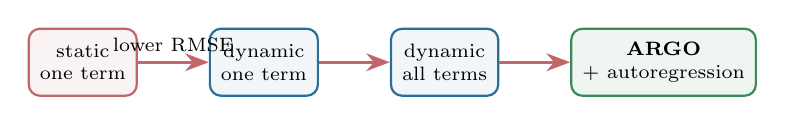
\begin{tikzpicture}[node distance=0.9cm]
    \node[rbox] (a) {static\\one term};
    \node[sbox, right=of a] (b) {dynamic\\one term};
    \node[sbox, right=of b] (c) {dynamic\\all terms};
    \node[gbox, right=of c] (d) {\textbf{ARGO}\\+ autoregression};
    \draw[flow] (a) -- node[above,font=\scriptsize]{lower RMSE} (b);
    \draw[flow] (b) -- (c);
    \draw[flow] (c) -- (d);
  \end{tikzpicture}}
  \end{center}
  \vspace{0.4em}
  \begin{itemize}
    \item Each upgrade is one honest, out-of-sample comparison on 2007--2011.
    \item Nothing here is a black box: you can read every coefficient and say what it does.
  \end{itemize}
\end{frame}

% ===============================================================
\section{Network approaches: ARGONet}

\begin{frame}{A location is not an island}
  ARGO uses one location's own search and history. But your \textbf{neighbors} carry signal
  too: what is rising next door often reaches you next (the mobility link from this morning).
  \begin{center}
  \resizebox{0.64\textwidth}{!}{%
  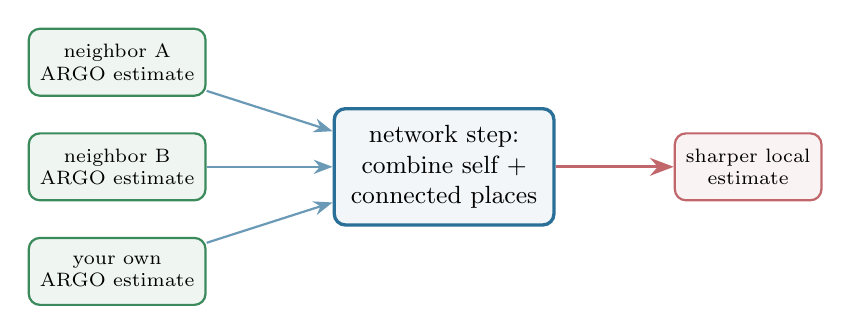
\begin{tikzpicture}[node distance=0.45cm and 1.4cm]
    \node[gbox] (n1) {neighbor A\\ARGO estimate};
    \node[gbox, below=of n1] (n2) {neighbor B\\ARGO estimate};
    \node[gbox, below=of n2] (self) {your own\\ARGO estimate};
    \node[cbox, right=1.6cm of n2] (net) {network step:\\combine self +\\connected places};
    \node[rbox, right=1.5cm of net] (out) {sharper local\\estimate};
    \draw[flowq] (n1) -- (net); \draw[flowq] (n2) -- (net); \draw[flowq] (self) -- (net);
    \draw[flow] (net) -- (out);
  \end{tikzpicture}}
  \end{center}
  \vspace{0.2em}
  \begin{itemize}
    \item \textbf{ARGONet} (Lu, Yang, Santillana et al., \emph{Nature Communications} 2019)
          adds a step that borrows strength from connected locations.
    \item There is a finer \textbf{county-level} version too. Same principle, more locations.
  \end{itemize}
\end{frame}

\begin{frame}{How the network step helps}
  \begin{itemize}
    \item Which neighbors? The ones with the most \textbf{shared movement} (the LODES /
          mobility ranking from this morning), or simply the most correlated at a short lag.
    \item Feed a neighbor's recent activity, or its ARGO estimate, in as an extra predictor,
          and let the dynamic fit decide how much to trust it.
    \item Where local data is thin or late, a well-connected neighbor can fill the gap.
  \end{itemize}
  \vspace{0.3em}
  \begin{center}
    \itshape The dengue CSV is one country, so this is a concept here; on the state or county
    panels it is a real, measurable gain.
  \end{center}
\end{frame}

% ===============================================================
\section{Wrap-up}

\begin{frame}{What you built}
  \begin{itemize}
    \item A single regression grown into \textbf{ARGO}: dynamic training $+$ selected search
          terms $+$ autoregression, validated out of sample at each step.
    \item A network idea (\textbf{ARGONet}) that borrows signal from connected neighbors.
    \item All of it \textbf{interpretable}, and all of it driven by prompts you can rerun for
          your own disease and place.
  \end{itemize}
  \vfill
  \begin{center}
    \itshape This is the operational machinery Candice runs weekly for Georgia flu. You just
    built the small version.
  \end{center}
\end{frame}

\begin{frame}{Looking ahead}
  \begin{itemize}
    \item \textbf{Next (Part 2, M. Santillana):} beyond flu monitoring in rich nations,
          emerging outbreaks, and weather as a modulator.
    \item \textbf{This afternoon (3:30):} the COVID exercise, detecting exponential growth in
          digital traces.
    \item \textbf{Day 3:} bring your own problem, and point ARGO at it.
  \end{itemize}
  \vfill
  \begin{center}
    \itshape From one search term and a straight line, to ARGO, in an afternoon.
  \end{center}
\end{frame}

\begin{frame}{Credits and sources}
  \footnotesize
  \begin{itemize}
    \item Exercise continues Mauricio Santillana's dengue exercise 2
          (\texttt{MIGHTE-lab/SISMID25}); data \texttt{MX\_Dengue\_trends.csv}.
    \item \textbf{ARGO:} Yang, Santillana \& Kou, \emph{Accurate estimation of influenza
          epidemics using Google search data via ARGO}, PNAS 2015.
    \item \textbf{ARGONet:} Lu, Yang, \ldots, Santillana, \emph{Improved state-level
          influenza nowcasting in the United States leveraging Internet-based data and
          network approaches}, Nature Communications 2019.
    \item Dynamic training as data assimilation; Lasso for term selection with many queries.
  \end{itemize}
\end{frame}

\begin{frame}[standout]
  Questions?\\[0.4em]
  \small Repo: \texttt{github.com/Shihao-Yang/sismid2026}
\end{frame}

\end{document}
